\documentclass[a4paper, 11pt]{article}
\usepackage[left=2cm, top=3cm, text={17cm, 24cm}]{geometry}
\usepackage[utf8]{inputenc}
\usepackage[czech]{babel}
\usepackage{graphicx}
\usepackage{verbatim}
\usepackage{enumitem}
\usepackage{times}
\usepackage[unicode]{hyperref}

\begin{document}

    \catcode`\-=12

    \begin{titlepage}
        \begin{center}
            {\Huge\textsc{
                        Fakulta informačných technológií \\
                        Vysoke učení technicke v~Brně \\
            }}
            \vspace{\stretch{0.382}}
            {\Large
                        \Huge {Projektová dokumentácia} \\
                        \LARGE {\textbf {Implementácia prekladača imperatívneho jazyka IFJ19}} \\
                        \vspace{\stretch{0.018}}
                        \large{Tým 033, varianta I}}
                        \vspace{\stretch{0.600}}
        \end{center}
    
        \hfill            
        \begin{minipage}[r]{0.49 \textwidth}
                \Large
                \begin{tabular}{l l l}
                    \textbf{Maroš Geffert} & \textless \textbf{xgeffe00}\textgreater & \quad 25\, \% \\
                    Patrik Tomov & \textless xtomov00\textgreater  & \quad 25\, \% \\
                    Martin Valach & \textless xvalac14\textgreater  & \quad 25\, \% \\
                    Andrej Pavlovič & \textless xpavlo00\textgreater  & \quad 25\, \% \\
                \end{tabular}
        \end{minipage}   
        
        \begin{minipage}[r]{0.4 \textwidth}
                {\Large \today}
        \end{minipage}    
        
    \end{titlepage}    
    
    
    %%%%%%%%%%%%%%%%%%%%%%%%%%%%%%%%%%%%%%%%%%%%%%%%%%%%%%%%%%%%%%%%
    \pagenumbering{arabic}
    \setcounter{page}{1}
    \tableofcontents
    \clearpage
    
    %%%%%%%%%%%%%%%%%%%%%%%%%%%%%%%%%%%%%%%%%%%%%%%%%%%%%%%%%%%%%%%
    \pagenumbering{arabic}
    \setcounter{page}{1}
    
    \section{Úvod}
    Cieľom nášho projektu bolo vytvoriť prekladač v~jazyku C, kotrý načíta zdrojový súbor zapísaný v~zdrojovom jazyku IFJ19, ktorý reprezentuje podmnožinu jazyka Python 3, a preloží ho do~cieľového jazyka IFJcode19. V prípade chyby vracia odpovedajúci chybový kód.
    
    \section{Implementácia}
    
    \begin{figure}[h]
		\centering
		\scalebox{0.45}{
			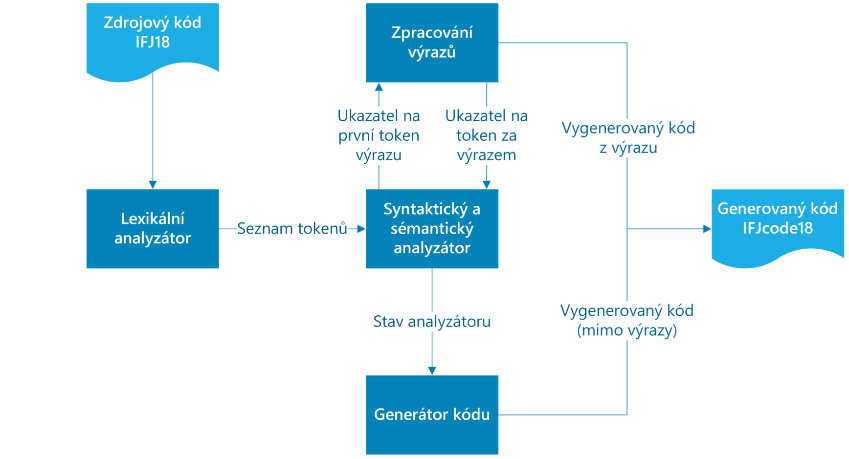
\includegraphics{inc/picture1.png}
		}
	\end{figure}
    
    \subsection{Lexikálny analyzátor}

    Pri programovaní prekladača, sme začínali s~tvorbou lexikálneho analyzátoru. Základnou funkciou tejto časti je funkcia \texttt{get\_token}, vďaka ktorej je možne načítávať lexémy\footnotemark zo~zdrojového súboru a~prevádzajú sa do~podoby takzvanej token. token je štruktúra ktorá obsahuje (atributy, typy, v~prípade identifikátoru si uchováva aj jednotlivý string atď.). Typy tokenov mǒzu byť klúčove slová, identifikator, rôzne operátory, EOL, EOF a~všetko čo jazyk IFJ19 podporuje. Jednotlive atributy sa k~tokenom priradzujú podľa situácie (napr. pre identifikátor, alebo čísla (float, integer).
    
    Lexikálny analyzátor funguje ako deterministický konečný automat. Tento konečný automat sme implementovali ako opakujúci sa switch, kde každý case odpovedá nejakému stavu z~automatu. Ak sa načítaný lexem nezhoduje so~žiadným odpovedajúcim stavom určeným jazykom IFJ19 tak vraciame chybu 1. Lexikálna analýza končí načítaním posledného znaku zo~zdrojového súboru, ktorým je \texttt{EOF} (Prípadne skončí v~chybovom stave pri~internej chybe). 

        
    \footnotetext{Lexéma je základná jednotka lexikálnej (čiže slovnej) zásoby jazyka, t.j. základná jazyková jednotka, ktorá je nositeľom vecného významu.}    
    \pagebreak    
        
    \subsection{Syntaktická analýza}
    
    Najpodstatnejšou časťou prekldača je syntaktická analýza tzv (parser). Parser je založený na~rekurzívnom zozstupe z~hora dolu. Jeho úlohou je kontrola, či reťazec tokenov reprezentuje syntakticky správne napísaný program. Pokial dojde pri~jeho činnosti k~chybe, vypíše sa kód chyby. Parser žiada tokeny od scanneru, kde potom na~základe tokenov pracuje s~tabuľkou symbolov.

    \vspace{4mm}
    
    \textbf{\large{Dvojprechodová}}
    \begin{itemize} 
        \item Naplnenie tabuľky symbolov funkciami
        \item Samotná analýza kódu
    \end{itemize}    
        
    \textbf{\large{Rekurzívny zostup}}
    \begin{itemize}
        \item Derivácia neterminálu na~zásobník
        \item Precedenčná LL(1) tabuľka
    \end{itemize}
    
        
    \subsection{Spracovanie výrazov}
    
    Dalšou častou prekladača je sémantický analyzátor. Pri~sémantickej analýze sa kontrolujú operácie nad dátovými typmi a~práca s~nimi (napr. ich pretypovanie). Jedná sa buď o~implicitnú konverziu alebo ošetreniu nepovoleného pretypovania. Všetky kontrolu sa robia na~základe dat, uložených v derivačnom strome, a~to pri~prechode stromom zdola horu.
        
    \subsection{Generovanie kódu}
    
    Generovanie kódu pre~nás znamená vytváranie medzikódu IFJcode19. Kód je generovaný na~štandartný výstup. Po dokončení všetkých analýz, pričom jednotlivé časti sú generované v~priebehu analýz do internej pamäti programu. Generátor vnútorného kódu na~základe naplnenej tabuľky symbolov generuje trojadresný vnutorný kód k~spracovaniu interpretom. Tento trojadresný kód sa generuje kvôli zjednodušeniu dalšej práce a~zjednodušeniu činnosti interpretu.
    
    \subsection{Interpret}
    
    Interpret vytvára interpretáciu trojadresného kódu, generovaného syntaktickým analyzátorom. Trojadresný kód je uloženy v~instrukčnom liste, ktorý je implementovaný pomocou jednosmerného viazaného lineárneho zoznamu. Pre každú inštrukciu je tento kód reprezentovaný typom inštrukcie, adresou výsledku a~adresami prvého a~druhého operandu. Pri spracovávaní aritmeticko-relačných operácií robí interpret sémantickú kontrolu.
    
    \pagebreak
    \section{Algoritmy}
    \subsection{Hash table}
    
    Hašovacia tabuľka je údajová štruktúra, ktorá asociuje kľúče s~hodnotami. Primárna efektívne podporovaná operácia je vyhľadávanie.
    
    \subsection{Dynamický string}
    
    Ďalší algoritmus, ktorý sme použili je \texttt{Lexem\_string} pre operácie s~reťazmi rôznej dĺžky. Štruktura má v~sebe uložene ukazatel na~reťazec, dĺžku reťazca a~aj kolko pamate je vyhradene pre~reťazec. Implementované operácie : inicializácia (Pri inicializácii sa vyhradí pamäť práve pre~určitý počet znakov a~ak je potrebne tak sa realokuje), uvolnenie dát, pridanie znaku alebo stringu do reťazca atd.
    
    \subsection{Tabulka priorít}
    
    
    
    \subsection{Tabuľka symbolov}
    
    Tabuľka symbolov predstavuje strom funkcií a~ukazateľ na práve používanu funkciu. Každá funkcia obsahuje strom premenných, zoznam konštánt a zoznam inštrukcií.
    
    \section{Práca v týme}
    
    Náš tým sa stretol po~zadaní projektu. Vedúcim týmu boli hneď aj rozdelené úlohy. Tím väčšinou medzi sebou komunikoval osobne alebo cez discord. 
    
    Najprv sme si stanovili štruktúru celého projektu. V~priebehu prvých šiestich týždňov sa toho veľmi neurobilo, implementoval sa lexikálny analyzátor, členovia študovali a~zbierali informácie ohĺadom svojej časti programu, ktorá im bola zadaná vedúcim tímu. V~priebehu ďalších týždňov sme implementovali celý program. Testovali sme jednotlivé časti osobitne, ale neskôr sme to už testovali spolu ako celok. K~zdielaniu kódu sa používal repozitár git.
    
    \begin{tabbing}
    meno ~~~~~~~~~~~~~~~~~~~~\= login ~~~~~~~~~~~
    \= rozdelenie práce \kill
    \bfseries Meno \>
    \bfseries Login \>
    \bfseries Rozdelenie práce \\[2mm]
    Maroš Geffert \> xgeffe00 \> Lexikálna analýza, dokumentácia, testy \\
    Patrik Tomov \> xtomov02 \> Syntaktická analýza\\
    Martin Valach \> xvalac14 \> Sémantická analýza \\
    Andrej Pavlovič \> xpavlo00 \> Generátor kódu
    \end{tabbing}


    \section{Záver}
    
    Projekt nás až tak nezarazil, vzhľadom nato, že sme sa naňho začínali pripravovať v~celku dosť skoro. Tím sme si zostavili veľmi rýchlo a~tým, že sme na~rovnakom internáte tak nebol problém s~akoukoľvek komunikáciou. Jednotlivé časti programu sme riešili z~väčšej časti individuálne.
    Správnosť projektu sme si overili automatickými testami a~pokusným odovzdaním, vďaka ktorému sme boli schopní projekt ešte viac doladiť.
    
    Na tomto projekte sme si vyskúšali implementáciu niektorých zaujímavých dátových štruktúr, algoritmov, teoriu formálnych jazykov v~praxi a~spoluprácu v týme.
    
    \clearpage
    
    \section{Digramy}
    \subsection{Deterministický konečný automat popisujúci lexikálnu analýzu}
    \begin{figure}[h]
		\centering
		\scalebox{0.5}{
			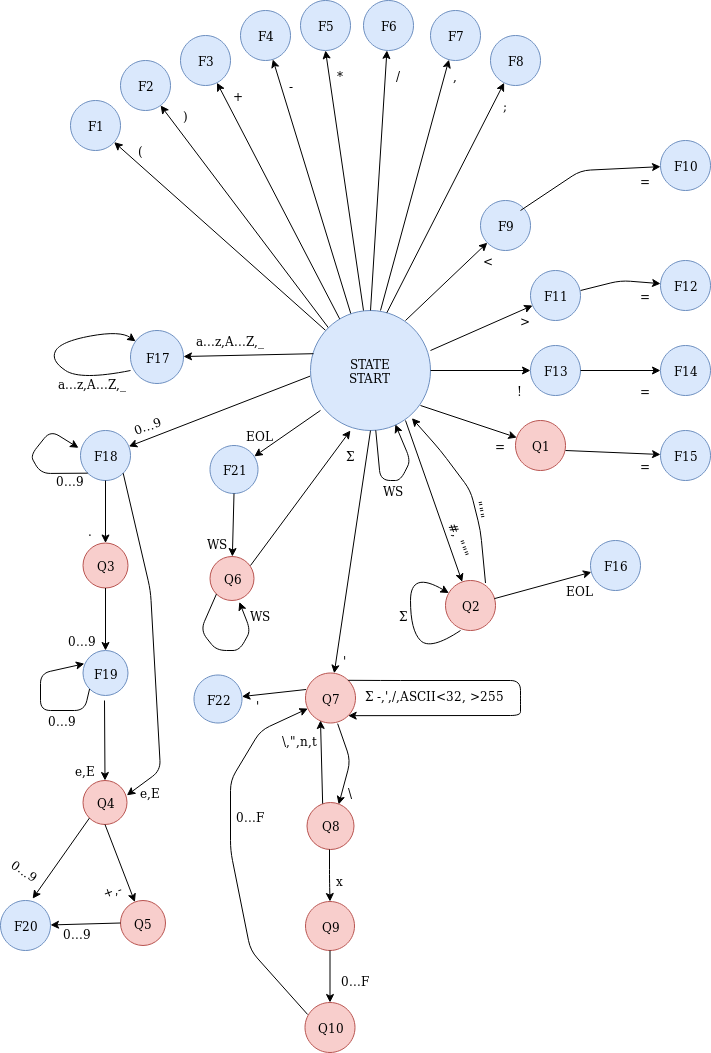
\includegraphics{inc/scannerAutomat.png}
		}
	\end{figure}

\end{document}
